\documentclass[12pt]{article}

\usepackage{graphicx}
\usepackage[margin=3cm]{geometry}
\usepackage{minted}

\graphicspath{ {./Imagenes/} }
\usemintedstyle{borland}

\begin{document}

\pagestyle{empty}

\section*{ Redacción del problema }

Envía un archivo PDF con el programa fuente que muestre una interfaz
gráfica con la distribución de border Layout en el JFrame y también en
el Panel central.  Coloque imágenes en las áreas norte,sur,este y
oeste del Jframe.

En el panel Central que también tiene la distribución de Border,
colocar etiquetas con los nombres de sus áreas
correspondientes. P.e. en el borde ubicado al norte colocar la
etiqueta "NORT".

Tu documento PDF, deberá contener tu hoja de presentación, la
redacción del problema, el código fuente de las clases que se usaron y
las capturas de pantalla que consideres a fin de mostrar el correcto
funcionamiento del programa.
\section*{ Código }

\subsection*{ Clase Gui }
\inputminted{Java}{./Gui.java}

\subsection*{ Clase de prueba }
\inputminted{Java}{./PruebaGui.java}

\section*{ Ejecución }
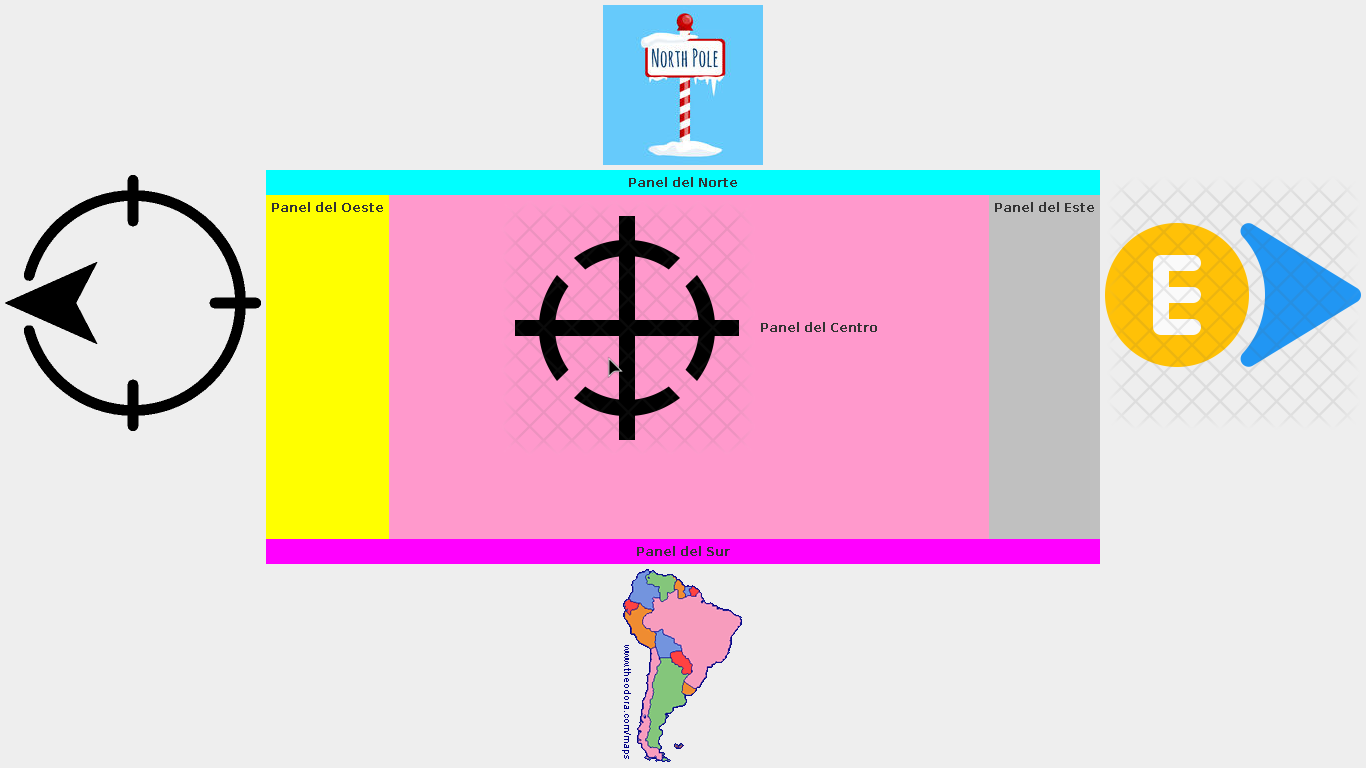
\includegraphics[width=\textwidth]{Corrida.png}

\end{document}
